
\doublespacing

%-------------------------------------------
%	Chapter 3: Track Reconstruction
%-------------------------------------------
\chapter{Track Reconstruction}
\label{chapter-3}

%H important to help show the bigger picture of my research and the motivation behind the work presented

%Successful particles physics measurements are dependent on an efficient and performant re- construction of the physics objects from the detector measurements. As a community we are always striving to run at the edge of the available detector and computation capabilities to ex- tract the maximum amount of information from the experiments. Tracking detectors are at the core of most collider experiments and track reconstruction is one of the crucial tasks in every reconstruction chain.

%Track reconstruction at its heart is a combinatorial problem, i.e. to find the measurements that originate from the same initial particle from a set of possible combinations. The created particles have a wide range of possible properties, especially different creation vertices and momenta, and their particle trajectories have non-deterministic contributions from material interactions. In combination with inhomogeneous magnetic fields and detector inefficiencies, this leads to the possibility of confusion, fake tracks, etc. . All of these effects depend strongly on the density of the measurements and thus on the collision pile-up. Consequently, with the upcoming upgrade to the High-Luminosity Large Hadron Collider (HL-LHC) the track reconstruction complexity will increase significantly.

In this chapter, track finding in silicon based detectors is presented. Section \ref{track-finding-silicon-trackers} outlines a typical workflow for track reconstruction in a multi-element silicon tracker and the parameterisation used for specifying the trajectory of charged particle tracks. Section \ref{ml-background} presents the theoretical formalism of a typical ML classification problem, as well as an introduction to the TrackML detector and its corresponding ML challenge. This section focuses on the realistic detector geometry used to simulate measured particle hits similar to those expected of the HL-LHC experiment, as well as the approaches and ideas to tackle the challenge of track reconstruction that arose from the challenge. Finally, graph network architectures and track reconstruction using graph networks is presented in Section \ref{graph-networks}, as a potential solution and optimisation to the track finding problem.


%The aim of this project is to explore track finding methods utilizing a graph-based track model and graph neural networks (GNN). An ML-based algorithm will be used to predict a graph adjacency matrix given the input hit features such as a shape of a charge cluster representing a track position measurement in a silicon detector. The excitation/inhibition rules of individual GNN neurons will be designed to facilitate the “simple-to-complex” approach for “hits-to-tracks” association such that the network starts with relatively “easy” areas of an event with low hit density and gradually progresses towards more complex “hot” areas. To efficiently exploit a priori knowledge about charged particle dynamics the GNN-based algorithm will be using simplified Kalman filters as mechanisms for information propagation and track extraction. 

% first talk about graph building using the ML hit pair predictor and then talk about graph pruning/track extraction using the GNN based algorithm



%--------------------------------------------------
%	Chapter 3: Track finding in Silicon Trackers
%---------------------------------------------------
\section{Track Finding in Silicon Trackers}
\label{track-finding-silicon-trackers}

%The reconstructed trajectories of charged particles are referred to as tracks. 
%Tracks are reconstructed from the energy depositions (called hits) left by the particles as they traverse the the inner detector.


Tracks are reconstructed from the energy depositions (\textit{hits}) left by the particles as they traverse the inner detector. Tracks are used in the reconstruction of other objects, including vertices and jets, so their accurate reconstruction is a critical task. A typical workflow for track finding in a multi-element silicon tracker (such as those in ATLAS and CMS) is given below and comprises a three-stage approach; seeding, track following, and track selection, implemented in many charged particle tracking algorithms and is commonly known as the \textit{inside-out} approach. A comprehensive introduction to ATLAS tracking is available in Ref \cite{Cornelissen:2007vba}.

%The main sequence is referred to as ’inside-out’ track finding, involving clusterisation [17], a CPU-expensive ’track-finding’, followed by precise estimation of track parameters via ’track-fitting’.


%--------------------------------------------------
%	Chapter 3: Track Reconstruction
%---------------------------------------------------
\subsection{Inside-Out Track Reconstruction}
\label{track-reconstruction}

%Describe a typical workflow for track finding in a typical multi-element silicon tracker such as ATLAS and CMS. This workflow is basically a three-stage approach with the seeding, track following, and track selection implemented in the current charged particle tracking algorithms. This is precisely the right place to introduce the TrackML setup. Add that the high-lumi LHC motivates the R\&D of new track finding techniques and we need an environment for fast prototyping and testing various techniques which would allow expert from outside HEP to contribute hence the TrackML.

%This section should be all about track finding in ATLAS, including the main pipeline outlining space-point formation (clustering), track finding (combinatorics), ambiguity solving, neural network cluster splitting, pattern recognition techniques, Kalman filters etc 


\subsubsection{Space-point Formation (Clustering)}
When a charged particle traverses a silicon layer, charge can be deposited in more than one pixel or strip. This is due to the incident angle of the particles with respect to the sensor and also the drift of electrons inside the sensor caused by their interaction with the magnetic field. Clusters are formed by grouping together neighbouring pixels or strips. The local position of the cluster on the sensor is typically estimated using the energy-weighted mean position of the pixels (or strips) forming the cluster. The clusters are then converted into 3D space-points by a coordinate transformation, where pixel space-points are identical to pixel clusters and strip space-points are formed by combining information from two strip clusters in subsequent sensors in the SCT (or strip double layers of the ITk).

\subsubsection{Seeded Track Finding}
Space-points are used to build track seeds. Seeds are defined as a group of three space-points located in different detector layers which are geometrically compatible with being part of a track segment. A combinatorial KF is used to build track candidates by extending track seeds. The filter searches for adjacent clusters both outwards and inwards in $r$ while attempting to smooth the trajectory. This method considers tracks as a sequence of hits and, from a particular starting point, will attempt to extrapolate throughout the detector collecting hits belonging to the same track. The filter can create multiple track candidates per seed, with bifurcations along the track occurring when more than one compatible space-point exists in a given detector layer. In this way, the filter creates an excess of track candidates, which are only required to satisfy basic quality requirements. Track candidates are allowed to share hits freely (a single hit may be used by multiple track candidates). Typically, the presence of shared hits is an indication of a bad track due to the high granularity of the ATLAS tracking detectors. At this stage, there can also be a large number of incorrect hits assigned to otherwise good tracks, and large numbers of fake tracks. Fake tracks are those where the majority of associated hits do not originate from the trajectory of any one physical particle. The end result of this track finding/pattern recognition process is a set of potential track candidates, generally of low quality, that then undergoes further refinement through an ambiguity resolution step in which the highest quality tracks are selected. The implementation of the filter approach in tracking is fast computationally, but is relatively imprecise and does not resolve ambiguities.

\subsubsection{Track Ambiguity Resolution}
\label{chapter-3-ambiguity-resolution}

The procedure so far has created candidates with potential overlap. In the ambiguity solver of the ATLAS detector, track candidates are processed individually in descending order of a track score in an effort to resolve this overlap. The track score quantifies the likelihood of the track corresponding to the trajectory of a real particle. Scoring uses a number of variables, including the number and positions of hits, the transverse momentum of the track and the fit quality described as the $\chi^{2}$ divided by the number degrees of freedom on the track. A preference for high transverse momentum tracks promotes the successful reconstruction of the more physically interesting energetic particles, and suppresses the large number of wrong hits assigned to low momentum tracks. The refined and purified track candidates resulting from the ambiguity resolution are re-fit using a global $\chi^{2}$ method in order to obtain the high-precision track parameter estimate. This accounts for errors on the measurements and expected uncertainties (e.g multiple scattering etc.) Ambiguity solving was introduced as part of the ATLAS New Tracking (NEWT) \cite{Cornelissen:2007vba} intended to improve track reconstruction performance in dense environments. 

\subsubsection{TRT Extension}
The successful tracks from the ambiguity solving stage are extended into the TRT. The TRT operates as a drift chamber: when a charged particle traverses a straw, the active gas mixture is ionised creating ionisation clusters.  The clusters are collected by applying a large potential difference between the wall of the straw and the wire. By measuring the time it takes the clusters to reach the wire, the distance of the track to the wire can be determined, and a valid set of matching drift circles can be formed. A road is then formed along the extrapolated track and the TRT drift circles that fall within this road are collected. Left/right ambiguities for the TRT drift circles are resolved and the output consists of the original tracks together with a list of associated TRT drift circles. A subsequent track refit is performed using the global $\chi^{2}$ fitter \cite{TGCornelissen2008}, in order to increase the precision in parameters of the reconstructed track. Unlike the KF, the global $\chi^{2}$ fitter is beneficial in its application in the TRT as it looks at all measurements at the same time and iteratively minimises the starting parameters. This differs from the KF, which determines the track state vector dynamically from measurements at each detector surface and requires a starting surface to proceed in its filtering. 

%In addition, the xenon gas in the straws is sensitive to transition radiation photons that are produced in the radiator material between the straws. As electrons produce many more photons than other particles through Bremsstrahlung, this difference is used in electron identification. 



% need to discuss this section in more detail, talk about the drift circles, bremstrahlung, using the global chi-2 fit to increase the resolution of pT and ....another parameter. how is the TRT included into the track fit. a global chi-2 refit is done, doesn't use the kalman filter, why? - motivate the chi2 fit


\subsection{The Outside-In Sequence}
The inside-out sequence of the ID, described in the aforementioned section, relies on a track seed to be found in the silicon detector. Although being very efficient, not all tracks can be found through an inside-out procedure: ambiguous hits can shadow the track seed in the silicon and prevent the score of the silicon seeded track to survive the ambiguity processor. In addition to this, tracks coming from secondary decay vertices further inside the ID volume or from photon conversions may not have any silicon hits (or only an insufficient number) to comply with the inside-out sequence. Clearly, when no candidate track in the silicon detector is found, the extension into the TRT is automatically lost. A second, reverse sequence has therefore been deployed that starts a global pattern recognition in the TRT. Track segments are identified using a standard Hough transform mechanism, while a dedicated association tool prevents hits that have already been assigned to tracks in the inside-out procedure to be used again (which saves a significant amount of CPU time).



%--------------------------------------------------
%	Chapter 3: Track Parameterisation
%---------------------------------------------------
\subsection{Track Parameterisation}
\label{track-parameterisation}

Tracks must be parameterised in order to extrapolate them to outer detector layers, to include further hits. There are several parameterisations of tracks, but since the shape of charged particle trajectories in a uniform magnetic field is helical, in general five parameters are required to approximate the true trajectory. One such parameterisation is known as perigee given by Eq. \ref{perigee}:

\begin{equation}\label{perigee}
\textbf{p} = (d_0, z_0, \phi, \theta, Q/p_T)
\end{equation}

The respective transverse and longitudinal impact pararameters; $d_0$ and $z_0$ specify the distance of closest approach of the trajectory of a particle to the nominal interaction point. $\phi$ is the azimuthal angle in the $x$-$y$ plane and $\theta$ is the polar angle in the $(r,z)$ plane. In fact, we often use $\cot(\theta)$ instead of $\theta$, since $\cot(\theta)$ is the inverse slope of the track. $Q/p_T$ is the inverse transverse momentum multiplied by the charge of the particle. The parametrised description of a particle trajectory is called a \textit{track model} (see Figure \ref{fig:track-parameters-perigee}).


\begin{figure}[!htbp]
  \centering
  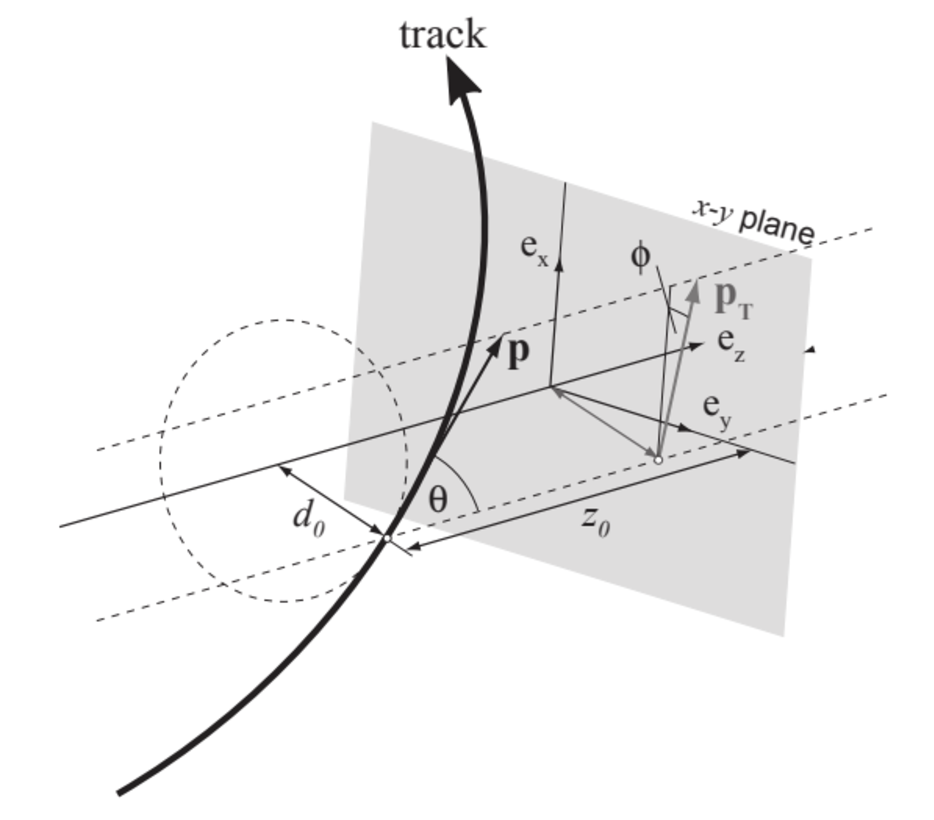
\includegraphics[width=0.65\textwidth]{images/3-track-reconstruction/track_params.pdf}
  \caption{Illustration of the perigee track parameters. Five coordinates are specified $(d_0, z_0, \phi, \theta, Q/p_T)$, defined at the track’s point of closest approach to the nominal interaction point at the origin of the coordinate system. The three-momentum \textbf{p}, transverse momentum $p_T$ and basis vectors $e_x$, $e_y$ and $e_z$ are also shown. Reproduced from Ref. \cite{atlastrackingdocs}
  }
  \label{fig:track-parameters-perigee}
\end{figure}






%--------------------------------------------------
%	Chapter 3: TrackML Model
%---------------------------------------------------
\section{Machine Learning in Track Reconstruction}
\label{ml-background}

\subsection{Machine Learning Background}

Over the past few decades, ML techniques have become increasingly prevalent in High Energy Physics experiments due the increased volumes of high-dimensional data and improvements in the field. Machine learning is the process by which a computer program uses data to learn suitable parameters for a predictive model. This is opposed to explicitly providing instructions on how to perform a task. A subfield known as \textit{supervised learning} is used in this work, and consists of exposing a model to a large number of labelled examples in order to extract relationships between the input data and their labels. These relationships are often complex, and explicitly programmed rules can fail to fully capture the relationships between inputs and outputs, as well as generalise to unseen data.

In the simplest case, a set of $n$ labelled training examples $S = \{(\textbf{x}_1, y_1), ..., (\textbf{x}_n, y_n)\}$ is collected. Each element $(\textbf{x}_i,y_i)$ consists of an input vector $\textbf{x}_i$ of dimension $m$, and the corresponding label $y_i$. In classification problems, typically $m$ is the number of unique features used to train the predictive model and the labels are integer class labels $y_i \in \{0,...,N − 1\}$, where $N$ is the number of categorical classes the training example belongs to (otherwise known as ground truth information). The rest of the discussion in this thesis is limited to binary classification problems ($N = 2$). Collecting sufficient and suitable data is one of the primary challenges of machine learning, as such data is not always readily available. Fortunately, sophisticated tools to simulate particle collisions have already been developed by the scientific community, one such example is in Ref \cite{Boos:2001cv}, as well as the others discussed further in Section \ref{trackml-simulation}. These tools play a key role in generating a suitably large amount of labelled data which is used to train algorithms.

After obtaining suitable training data, the next step is to define a model. Given an input domain of dimension $m$ and an output domain (0, 1), the model $f_{\theta} : \mathbb{R}^{m} \to (0, 1)$ is a parameterised functional mapping from input space to output space. Given an input example $\textbf{x}_i$ and a set of parameters $\theta$, the model outputs a prediction $\hat{y}_i \in (0, 1)$ for the true label $y_i$, as in:


\begin{equation}
    f_{\theta}(x_i) = \hat{y}_i
\end{equation}

The output $\hat{y}_i$ is in the interval (0, 1) so as to be interpreted as the probability that the input example $\textbf{x}_i$ belongs to class 1, commonly referred to as the $signal$ class. The parameters $\theta$ of the model are typically optimised and the model is designed to be expressive enough to correctly map the inputs $\textbf{x}_i$ to the outputs $y_i$. To perform this optimisation, the model is trained, which amounts to showing the model a series of labelled training examples and modifying the parameters of the model based on its ability to correctly predict the labels and maximise commonly used metrics. See Chapter \ref{chapter-4} for a detailed construction of a ML classifier.

\subsection{The TrackML Model}
\label{trackml-detector}

As the CPU time to reconstruct particle trajectories from measurements is expected to increase faster than the projected computing resources for future detector upgrades, new approaches to pattern recognition are needed to fully exploit the discovery potential of modern silicon detectors. In order to acquire an environment for fast prototyping and developing various techniques, a realistic detector model is needed. As a result, in 2018 a tracking ML challenge was organised on the Kaggle platform; an open-source community platform for data scientists dedicated to the use of challenges as a research tool. The \textit{TrackML Particle Tracking Challenge} \cite{kaggle-trackml} was held in an effort to spark new ideas and algorithmic approaches towards track reconstruction. The basis of the challenge is, using a realistic detector model, develop an algorithm for tracking trajectories of particles using machine learning techniques. The TrackML model simulates measured particle hits similar to those expected for a HL-LHC experiment and the corresponding data contains 8000 events to train on, where each event has up to 100,000 hits. The participants of the challenge were tasked with connecting these hits into approximately 10,000 arcs of circles, following the trajectory of particles issued from truth data from high energy proton collisions. 

There are many different approaches explored within the TrackML challenge, where the definition of a track determined the most effective approach to use. For example, for a track defined as a point-like object in a parameter space, clustering algorithms would be most appropriate. Whereas, for a track modelled as a sequence of hits, a track following algorithm using an iterative predict and update mechanism would be most effective. The structure of the TrackML detector is shown in Section \ref{trackml-structure}, the simulation of the model is discussed in Section \ref{trackml-simulation} and a summary of the challenge algorithms that are beneficial for this thesis is presented in Section \ref{trackml-key-findings}. The TrackML detector is also used for the development of the GNN-based algorithm; see Chapter \ref{chapter-6} for further information. More information on the TrackML challenge can be found in \cite{Amrouche_2019}.

\subsection{TrackML Detector Structure}
\label{trackml-structure}
The structure of the detector adopts a generic tracker design that takes key concepts from the existing proposals from ATLAS and CMS detectors. Many modern particle detectors include extensive silicon tracking systems arranged in thin layers of silicon sensors. The TrackML detector is very similar in structure to that of modern detectors, such as the ATLAS ITk \cite{inner-detector-TDR} being built for the HL-LHC era. It uses a cylinder-like geometry in the central regions and a disk-like geometry in the forward regions. The full TrackML detector geometry is shown in Figure \ref{fig:trackml-detector-image}. 


\begin{figure}[!htbp]
  \centering
  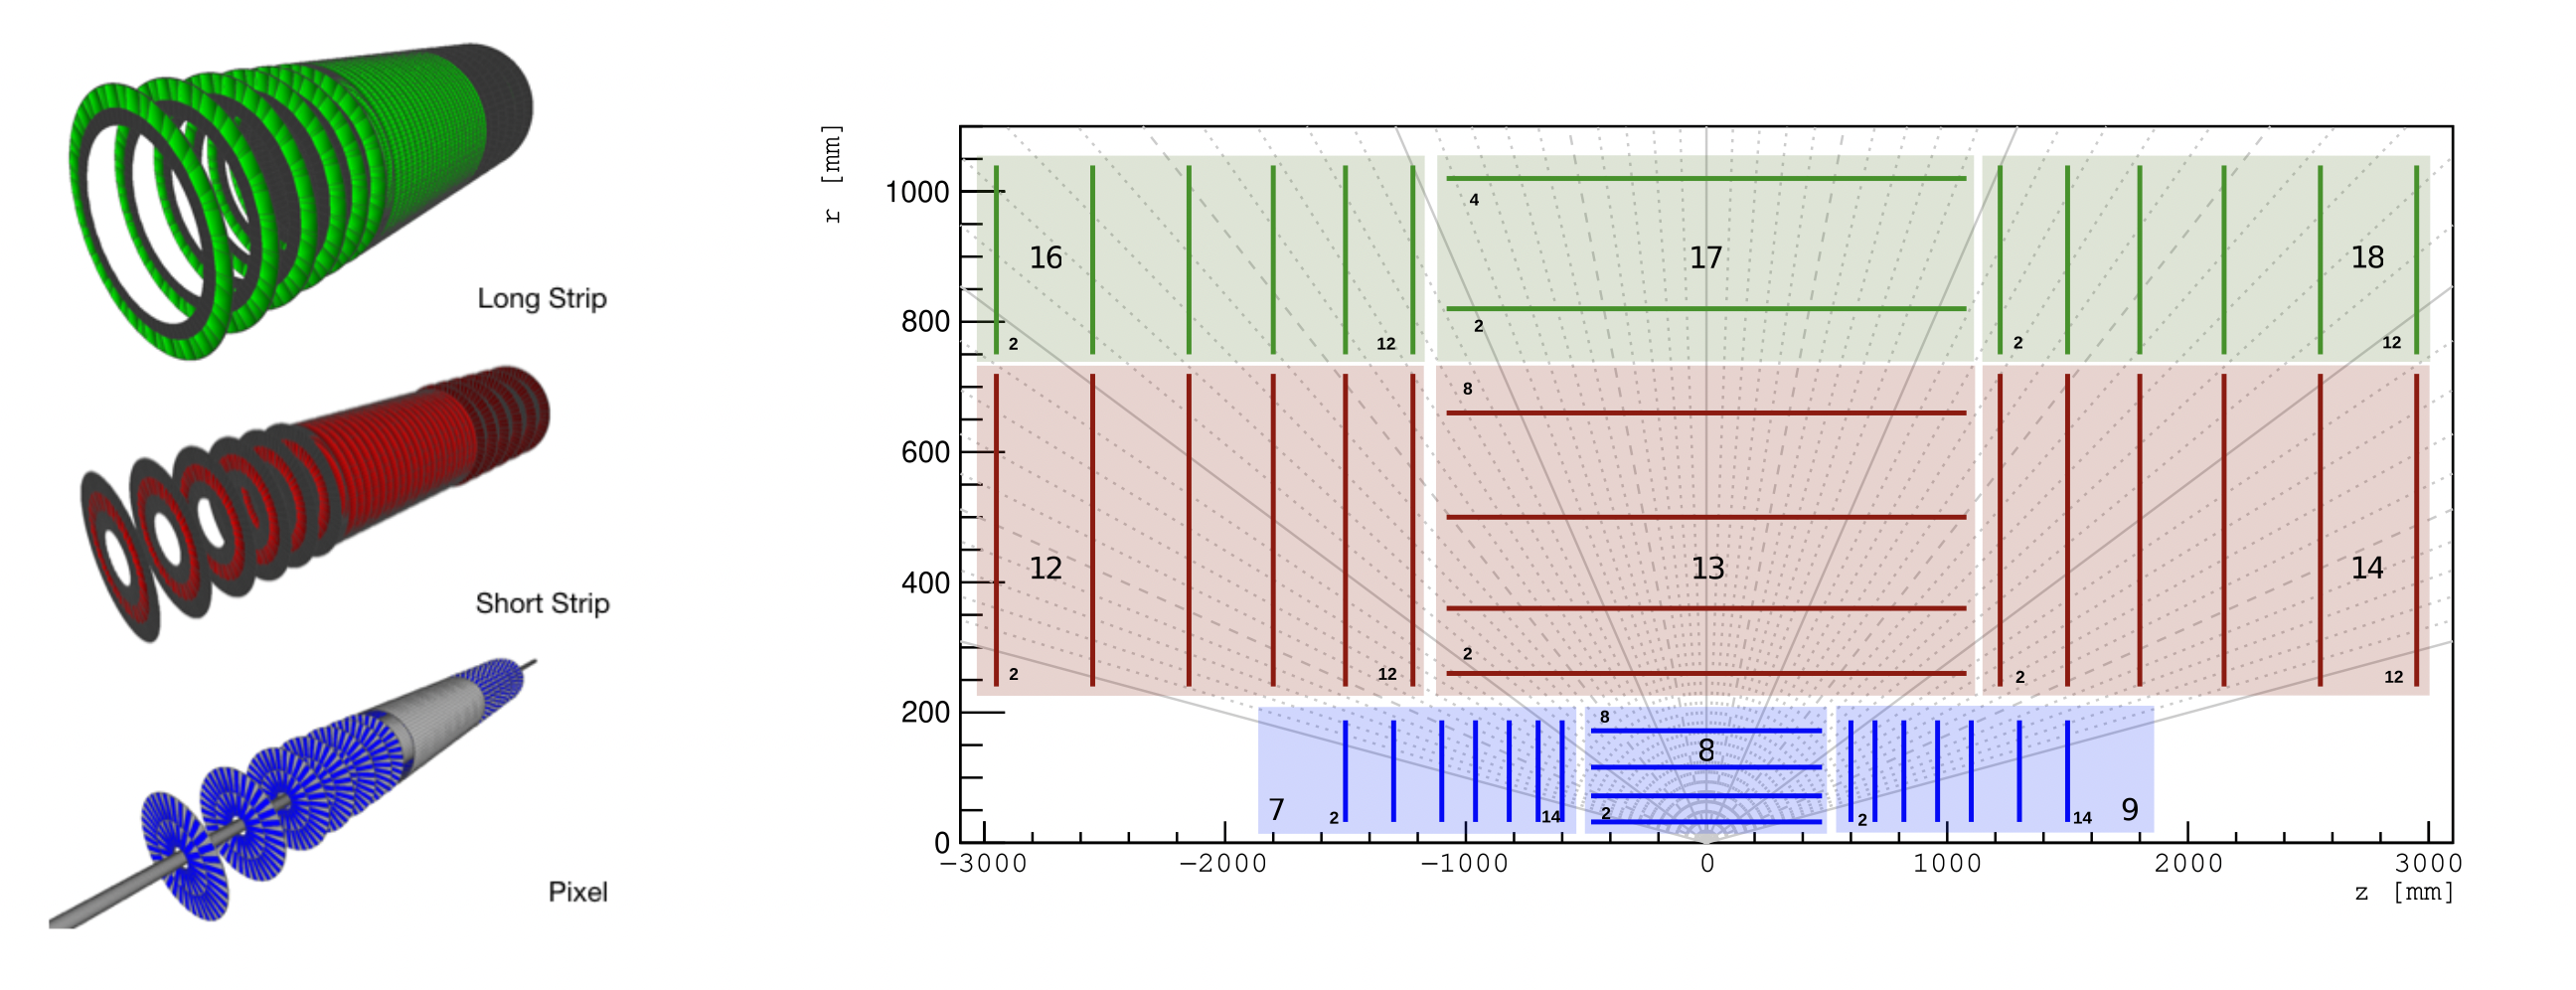
\includegraphics[width=\textwidth]{images/3-track-reconstruction/trackml-detector.png}
  \caption{
    Detector layout for the virtual TrackML detector. On the left the three major sub-detectors, pixel, short strips, and long strips, are shown separately. On the right, a schematic of the full layout and its coverage along the radial and longitudinal dimensions as well as in the $ \lvert \eta \rvert$ direction is shown. The different colors represent the different sub-detectors while the marked numbers are the internal volume and layer identifiers.
  }
  \label{fig:trackml-detector-image}
\end{figure}



The detector is split into three separate sub-detectors that differ in spatial resolution and passive material. The innermost sub-detector is a pixel detector with a spatial resolution of 50 $\mu$m $\times$ 50 $\mu$m and further out two different strip detectors with short 80 $\mu$m × 1200 $\mu$m and long strips 0.12 mm $\times$ 10.8 mm are placed. Each detector includes realistic module geometries with placement and overlap chosen to yield a hermetic coverage up to $\lvert \eta \rvert$ = 3. The particle beams collide on the $z$-axis around z = 0 mm. This is the centre of collision and also the centre of the detector. The TrackML detector is also organized into groups of layers, called \textit{volumes}, which are identified by a volume number. The pixel detector is represented by volumes 7, 8 and 9.

%ITK: There is no reason to believe the more complex geometry would lead to radically different algorithms

%The TrackML detector also shares several interesting features with the ATLAS detector, for example its solenoid parameters are the same and ....

%Instead of using the proposed upgrade tracker designs of either ATLAS or CMS we opted to design a generic tracker design that takes the key concepts from the existing proposals. This avoids issues of private collaboration information or artefacts and allows a challenge that is more separated from the particular design choices made by each experiment.

% -------------------------------
%More details in the documents on the TrackML competition:
%https://hal.inria.fr/hal-01745714/document
%https://arxiv.org/pdf/1904.06778.pdf
% ------------------------------


\subsection{Event Simulation}
\label{trackml-simulation}
%10.1051_epjconf_201921406037.pdf
The particle content of the collisions is generated using the Pythia 8 event generator \cite{pythia-8}. Pythia is a standard tool for generation of high-energy collisions, and contains a library to model hard scatter processes as well as the initial and final state of parton showers. A hard Quantum Chromodynamic (QCD) interaction that generates a $t\bar{t}$-pair (top quark and top antiquark) is used as the signal. An additional $\langle \mu \rangle$ = 200 soft QCD interactions (Poisson distributed) are overlayed to simulate the expected pile-up conditions at the HL-LHC. Charged particles are propagated through the detector using a fast detector simulation based on the ACTS software \cite{Gumpert_2017}. A non-homogeneous magnetic field is used, similar to the one in ATLAS, and material interactions, i.e. multiple scattering, energy loss, and hadronic interactions, are simulated using parametric models. Only tracks with a transverse momentum above 150 MeV are propagated. Tracks below this momentum threshold are typically not considered by the HL-LHC experiments.

% top quark decays: https://en.wikipedia.org/wiki/Top_quark

\subsection{Challenge Summary and Outlook}
\label{trackml-key-findings}

The TrackML competition exposed a diverse range of ML approaches, where accuracy and throughput were used to categorise the best algorithms for track reconstruction. The performance of the algorithms are evaluated using track purity and particle purity, for tracks originating from primary particles produced in the actual pp collisions. The purity is defined as follows; each track is matched with the ground truth majority particle sharing with it the greatest hit number, $N_{truth}$. The ratio of $N_{truth}$ to the number of hits of the reconstructed track, $N_{hits}$, defines the track purity, while the ratio of $N_{truth}$ intersection to the number of hits of the underlying particle, $N_{phits}$, defines particle purity. The quality of the top performing algorithms were analyzed in further detail. It was found that methods based on track following techniques are highly effective at reconstructing tracks globally with high purity, in comparison with clustering based approaches. 

Amongst the top ranking solutions, the developed algorithms were highly inspired from traditional track following approaches, such as the procedure outlined in Section \ref{track-reconstruction}. A short review of the submitted solutions that are influential to the research presented in this thesis is provided.

\subsubsection{TopQuarks Algorithm}

The winning algorithm proposed by the \textit{TopQuarks} team is based on a modular track following strategy, where the definition of a track is given by a sequence of hits. It begins with seed generation selected from hit pairs (doublets) in the innermost layers of the detectors. A logistic regression classifier is trained on doublet features and allows to reduce the number of fake seeds. The logistic classifier typically utilises the sigmoid function taking input and classifying it as a continuous output, representing the probability of good doublet prediction. The doublets are then extended to triplets via a further logistic classifier trained on triplet features. Track following is then implemented using a helix extrapolation and track ambiguity resolution is executed to remove polluting hits. The TopQuarks solution achieved approximately 95\% track reconstruction efficiency during the accuracy phase of the competition, with both its track purity and particle purity defined as $> 50\%$, as per the competition definition.

% Tracks are then consolidated by taking into account any hits located on overlapping modules if they are closer than a defined threshold.

\subsubsection{Outrunner Algorithm}

Another high-ranked algorithm is proposed by the \textit{Outrunner} team, based on training a multi-layered perceptron (MLP) to predict whether any two hits that are connected to the same track, where the definition of a track is the same as above. All pairs of hits were considered and 27 input features were constructed from its quantities. A neural network model composed of multiple wide dense layers is trained to predict the probability of the pair to be on the same track, hence predicting the adjacency matrix of network connections. The proposed approach is an unstructured track following algorithm where the next hit is not provided by track extrapolation, but directly by a hit index based on the hit pair classifier score. This suggests that too many branches of the combinatorial tree are followed during the track following step. The Outrunner solution achieved $> 90\%$ track reconstruction efficiency during the accuracy phase of the competition, and both its track purity and particle purity defined as $> 50\%$, as per the competition definition.

% There is a large class imbalance in the problem due of the predominance of pair of hits that are not belonging to the same track. This is overcome by sampling pairs from the negative class closer to the positive pairs to better define the boundary between the two classes. The accuracy weighted by the class cardinal is a better estimator of the performance of the model in this heavy imbalanced setup.

\subsubsection{Other Proposed Solutions}

Another team used various techniques based on the famous clustering-based approach DBSCAN (Density-Based Spatial Clustering of Applications with Noise) \cite{dbscan}. The idea of the DBSCAN-based algorithm was to find a subspace of track parameters in which a good track could be represented as a point-like object in this subspace. It is a popular clustering algorithm used commonly in data analysis and pattern recognition. It groups data points based on their density, identifying clusters of high-density regions and classifying outliers as noise. Track candidate building is executed using doublet track parameters, such as curvature and longitudinal impact parameters, within the DBSCAN clustering. This type of transform is a highly complex task and despite a best effort, the proportion of good tracks reconstructed was $\simeq$ 50\%. 

An alternative methodology implemented by another team utilises a Recurrent artificial Neural Network (RNN) using Long Short-Term Memory cells (LSTM). In contrast to uni-directional feed-forward neural network, RNNs are bidirectional, meaning that they allow the output from certain nodes to affect subsequent input to the same nodes. Their ability to use internal state (memory) to process arbitrary sequences of inputs makes them applicable to tasks such as sequence data. The LSTM mechanism provides a short-term memory for the RNN that can last thousands of timesteps, and as such RNNs can keep track of arbitrary long-term dependencies in the input data. The ability of RNNs to capture temporal dependencies makes them well-suited for tasks such as language modelling and sequential data analysis. Both RNNs and GNNs exploit a similar processing framework, but they can be applied to different input domains. Typically, RNNs require the input graphs to be directed and acyclic, whereas GNNs can process any kind of graph structure, making them versatile in nature and applicable to more complex problems.

The proposed solution to the TrackML challenge begins with seed building, where the DBSCAN algorithm is used to cluster hits in the inner-most layers of the detector in order to produce tracklet seeds. The RNN is then used within the path prediction stage in place of a propagator (such as a traditional KF track following algorithm) to find the potential position of hits on subsequent layers of the detector. The RNN model is trained using multiple architectures and used to predict the positions of the next hits, however the training of the models is quite prohibitive to allow for a full optimization due to its computational load. The proportion of good tracks reconstructed from this algorithm was $\simeq$ 85\%. More information about the details of the competition criteria, analysis and algorithm breakdown can be found in \cite{Amrouche_2019}.


\subsubsection{Motivation for Graph Neural Network Approach}
Several approaches highlighted by the TrackML challenge show great promise for accurate track reconstruction. However, in realistic detector setups, the physics reach of particle detectors will be limited by how efficiently the experiments can use their available computing resources. Many of the teams which applied deep learning to the vast amount of training data in the challenge faced computation resource limitations. Even with the use of general purpose Graphical Processing Units (GPUs), training of the models took multiple days. These approaches would not be suitable to implement in the software for realistic detectors.

In addition, approaches that heavily rely on the use of clustering are also not effective for realistic detectors. Clustering-based techniques require finding a parameter space where tracks exist as point-like objects. If a detector model contained a perfect uniform magnetic field and there were no material effects present, the behaviour of tracks in such a parameter space could be easily modelled as points and hence algorithms such as DBSCAN would be highly effective. However, this is not the reality due to multiple scattering effects. Clustering-based approaches are widely used to combine hits into doublets and extend doublets to triplets, however they are not the most successful when used to reconstruct tracks globally. The above factors were considered when exploring an alternative route. 

In recent years, algorithms for track pattern recognition based on GNNs have emerged as a particularly promising route. The authors of Ref. \cite{farrell2018novel} identified the use of GNNs as a promising solution for charged particle tracking at the HL-LHC. Since this publication, significant effort has been invested in the development of algorithms based on GNNs. One method in particular focuses on establishing a method based on training MLPs and employing deep learning techniques through GNN application and is the work done by the Exa.TrkX project \cite{ExaTrkX-website, Caillou:2815578}. Excellent performance of this GNN-based algorithm on the TrackML dataset \cite{refId0} has been demonstrated in Ref \cite{Ju_2021} and further information on this application is discussed in Section \ref{track-recon-graph-networks}. In contrast to the approach taken by the Exa.TrkX project, presented in this thesis is a novel methodology developed for track reconstruction using GNNs, without employing deep learning techniques. Prior to presenting this approach, an introduction to graph network architectures is given in Section \ref{graph-networks}.


%From the ML point of view, the problem can be treated as a \textbf{latent variable problem} similar to clustering, in which particle trajectory “memberships” must be inferred, a \textbf{tracking problem} considering trajectories as time series, or a \textbf{pattern de-noising problem} considering that the dotted trajectories are noisy versions of continuous traces. As a result the competition exposed a diverse range of ML approaches.

% One important point is that the points on one trajectory are not geometrically close to each other (a human cannot associate the points by eye), but they follow a specific pattern : a distorted arc of helix pointing approximately to the origin.

% Tracking efficiency is commonly defined in particle physics as the probability to reconstruct a track. A good tracking algorithm must provide consistently high efficiency over a wide range of track parameters.


%--------------------------------------------------
%	Chapter 3: Graph Networks
%---------------------------------------------------
\section{Graph Network Architectures}
\label{graph-networks}

Graph network structures are data representations that describe objects and their pairwise relationships. Graphs are able to effectively capture complex relationships and dependencies between such objects, both on a local scale and globally. This is essential for accurately representing physical data and understanding the interactive behaviour of the network. As a result, GNNs can represent many types of relational and geometric data. Due to their great expressive power, GNNs have been applied in numerous different applications. They have emerged as the de facto standard for many geometry-heavy applications, such as molecular property prediction within drug discovery and social network analysis.

As graph-based architectures are a natural way to represent tracks, they have shown substantial promise for a variety of particle physics tasks. This includes track reconstruction and simulation. Section \ref{properties-graph-networks} presents the properties and common terminology used within the domain of graphs networks and Section \ref{track-recon-graph-networks} compares the track reconstruction methodology developed in this thesis, with a similar approach by the Exa.TrkX collaboration.

%In some cases, GNNs have demonstrated better scaling properties, reduced resource utilization and increased opportunity for parallel implementation compared to traditional methods.

% Useful links!!
% https://www.datacamp.com/tutorial/comprehensive-introduction-graph-neural-networks-gnns-tutorial
% https://distill.pub/2021/gnn-intro/


%--------------------------------------------------
%	Chapter 3: Properties of graph networks
%---------------------------------------------------
\subsection{Properties of Graph Networks}
\label{properties-graph-networks}

%\subsubsection{Graph Network Architecture}

A graph $\mathcal{G}$ is defined by a set of \textit{nodes} \{V\} (or vertices) and a set of \textit{edges} \{E\}. Nodes represent entities or objects and edges are connections between two nodes that model their pairwise relationship. These edges can be directed, non-directed and/or weighted, see Figure \ref{fig:graph-architecture-example} for example illustrations. The connectivity of a graph can be visualized through its adjacency matrix $A \in \{0, 1\}$, of size $n_{nodes} \times n_{nodes}$. If two nodes share an edge, then the corresponding entry in the adjacency matrix is populated with 1, and zero otherwise. 

The data from a tracking detector for a given event can naturally be represented using a graph. A node can represent a hit (or a group of close proximity hits) with each node containing attributes such as spatial coordinates, and the existence of an edge between two nodes indicates that the nodes could potentially represent two successive hits on a track. At the HL-LHC, $O(10^{5})$ hits per $t\bar{t}$ event are expected. A fully connected graph of such an event would have $O(10^{10})$ edges, most of them representing unphysical connections. Therefore, a key feature within graph construction is the choice of compatible edges. 

\begin{figure}[!htbp]
  \centering
  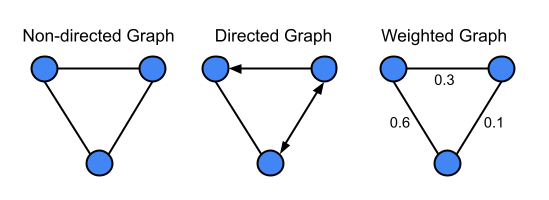
\includegraphics[width=0.85\textwidth]{images/3-track-reconstruction/Graphs.png}
  \caption{
    Illustration of different graph types. Non-directed graphs contain edges with no direction. Directed graphs can contain edges with unidirectional or bidirectional edges. Weighted graphs associate a weight to each edge, the example above has normalised edge weights. All three graphs are fully connected, whereby a unique edge connects each pair of nodes.
  }
  \label{fig:graph-architecture-example}
\end{figure}


\subsubsection{Message Passing Paradigm}

Message passing is an important property in the design of graph networks. It allows the propagation of node features by exchanging information between adjacent nodes. The edges between nodes act as conduits, allowing the transfer of information in a given direction if the connection is active. Typically, this scheme is iterative in nature. It begins with an initialization of a state at each node in the network, where a state typically comprises node or edge features. The node, $v$, then aggregates states from adjacent nodes in its local neighbourhood. Node representations are then updated based on an aggregation function, improving the precision of states local to each node. This process is then repeated with further message passing and neighbourhood information aggregation, allowing local information to spread globally throughout the network. GNNs can fully exploit the connectivity of their structure, and as a result the mechanism allows models to become sophisticated in learning rich and expressive representations of nodes that incorporate both local and global behaviour.


%--------------------------------------------------
%	Chapter 3: Track reconstruction on graph networks
%---------------------------------------------------
\subsection{Track Reconstruction using Graph Networks}
\label{track-recon-graph-networks}

The ExaTrkX collaboration \cite{ExaTrkX-website} has proposed an approach for track reconstruction using GNNs \cite{Caillou:28155782}. This graph-based algorithmic pipeline has two main stages, the first being graph construction and the second being track finding. Their approach represents a particle collision as a collection of nodes and edges. Each hit is treated as a node, which encodes features such as spatial position, and nodes are connected by edges that represent the possibility of two nodes belonging to the same track. Their goal is to use ML and graph techniques to segment or cluster the nodes to match particle tracks. The construction of the graph network is executed by training a MLP for edge classification by predicting edge scores, where message passing is used within the network to improve the discrimination power of the classifier, as well as a metric learning approach. Track finding is then done through deep learning approaches by training the GNN, as well as a graph segmentation process utilizing connected components and edge classification.

The proposed approach by the ExaTrkX project requires the use of deep learning techniques, which can result in the enormous use of computational resources. Considering the work developed by ExaTrkX, as well as the ideas which stemmed from the TrackML challenge, this has inspired the research presented in this thesis. 

Showcased here is a novel methodology exploring the use of a GNN architecture as a solution to the track pattern recognition problem, without the use of traditional deep learning techniques. The procedure developed here is somewhat of an intermediary of the described algorithms submitted to the TrackML challenge in Section \ref{trackml-key-findings}, as well as the incorporation of new techniques. The GNN-based model presented in this thesis is used to model tracks as sequences of points in a parameter space and simultaneously allows the natural structure of particle trajectories to be embedded into its architecture. 

There are two main aspects to this approach; a procedure to construct a graph network is presented in Chapter \ref{chapter-4} and a method to refine its connections and extract tracks is presented in Chapter \ref{chapter-5}. In order to identify compatible connections, a ML-based algorithm is used to predict if two hits belong to the same track, given input hit features, such as the charge distribution in the cluster. The training involved in this procedure is such that functions used to calculate track state parameters are learned, without using deep learning or vast computational resources. This approach ensures a realistic implementation for detector experiments. Following this, an iterative procedure allows ambiguities in the network to be identified and tracks to be isolated. To efficiently exploit a priori knowledge about charged particle dynamics the GNN-based algorithm uses simplified KFs as mechanisms for information propagation as well as for track extraction. Further information is given in Chapters \ref{chapter-4} and \ref{chapter-5}.